\chapter{Temps propre, dilatation du temps et contraction des longueurs}

Nous choisirons souvent des unités dans lesquelles la vitesse de la lumière vaut $c=1$. Dans ces unités, on peut comparer directement une année de temps à une année-lumière de distance, et les formules sont beaucoup plus lisibles. Chaque fois que $c$ intervient physiquement, nous le rétablissons. L’analyse dimensionnelle suffit à le retrouver.

\section{La grille galiléenne de l’espace-temps}

Commençons par la relation pré-einsteinienne entre un référentiel au repos et un train qui se déplace à la vitesse $v$ le long de l’axe $x$ :
\begin{align}
x' &= x-vt, & t'&=t.
\label{eq:l4-galilean}
\end{align}
La deuxième équation exprime l’hypothèse newtonienne d’un temps universel. Tous les observateurs utilisent les mêmes tranches de simultanéité, même si leurs origines spatiales sont en mouvement l’une par rapport à l’autre.

Supposons que l’observateur non primé se trouve à côté de la voie ferrée et que l’observateur primé voyage dans le train. L’origine du train a pour coordonnée $x'=0$ ; sa ligne d’univers dans les coordonnées non primées est donc
\begin{equation}
x=vt.
\end{equation}
Cette droite inclinée est l’axe $t'$. En revanche, $t'=t$ signifie que toutes les lignes de valeur constante de $t'$ sont les mêmes droites horizontales que celles de valeur constante de $t$.

\begin{figure}[H]
\centering
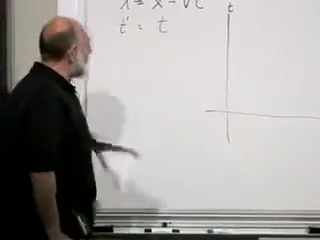
\includegraphics[width=0.72\textwidth]{lecture_04_figure_02.png}
\caption{La transformation galiléenne et la grille initiale $t$-$x$. L’origine mobile décrit $x=vt$, tandis que les deux référentiels conservent des lignes de temps constant communes.}
\lectureframe{00:03:06}
\end{figure}

En résolvant l’équation~\eqref{eq:l4-galilean} par rapport aux coordonnées non primées, on obtient
\begin{align}
x&=x'+vt'=x'+vt, & t&=t'.
\end{align}
La transformation inverse a la même forme, avec $v$ remplacé par $-v$. Si le train avance par rapport à la gare, la gare recule par rapport au train. Cette réciprocité subsiste en relativité restreinte, contrairement au temps universel.

\section{La correction de Lorentz}

Les transformations galiléennes ne peuvent pas rendre la vitesse de la lumière identique dans tous les référentiels inertiels. Les relations corrigées s’écrivent d’abord dans les unités où $c=1$ :
\begin{align}
x'&=\frac{x-vt}{\sqrt{1-v^2}}, &
t'&=\frac{t-vx}{\sqrt{1-v^2}}.
\label{eq:l4-lorentz-natural}
\end{align}
En rétablissant les unités usuelles, on obtient
\begin{align}
x'&=\frac{x-vt}{\sqrt{1-v^2/c^2}}, &
t'&=\frac{t-vx/c^2}{\sqrt{1-v^2/c^2}}.
\label{eq:l4-lorentz-c}
\end{align}

\begin{figure}[H]
\centering
\includegraphics[width=0.74\textwidth]{lecture_04_figure_05.png}
\caption{La transformation de Lorentz avec les facteurs de $c$ rétablis.}
\lectureframe{00:09:10}
\end{figure}

Pour $v\ll c$, $v^2/c^2$ et $vx/c^2$ sont tous deux très petits dans les situations où l’on utilise la mécanique newtonienne. L’équation~\eqref{eq:l4-lorentz-c} se réduit alors au résultat galiléen. La relativité n’abandonne pas la cinématique newtonienne ; elle en délimite le domaine de validité.

Pour $v=c$, le dénominateur s’annule. Un référentiel inertiel ne peut pas se déplacer à la vitesse de la lumière par rapport à un autre référentiel inertiel. Bien en dessous de cette limite, les corrections sont faibles, mais à proximité, le mélange de $x$ et de $t$ devient inévitable.

Le mouvement étant choisi selon $x$, les coordonnées transversales ne changent pas :
\begin{equation}
y'=y,\qquad z'=z.
\end{equation}
On peut comprendre pourquoi en plaçant des règles identiques dans la direction transversale, l’une dans le train et l’autre sur le quai. Un observateur se déplaçant à mi-chemin entre les deux référentiels voit les règles s’approcher à des vitesses égales et opposées. Rien dans cette configuration ne peut faire paraître l’une des règles transversales plus courte que l’autre.

\section{Transformations de Lorentz le long du cône de lumière}

L’équation~\eqref{eq:l4-lorentz-natural} se prête à une lecture géométrique. Additionnons ses deux équations :
\begin{align}
t'+x'
&=\frac{(t-vx)+(x-vt)}{\sqrt{1-v^2}}\\
&=(t+x)\frac{1-v}{\sqrt{1-v^2}}\\
&=(t+x)\sqrt{\frac{1-v}{1+v}}.
\label{eq:l4-null-plus}
\end{align}
Soustrayons-les dans l’ordre inverse :
\begin{align}
t'-x'
&=\frac{(t-vx)-(x-vt)}{\sqrt{1-v^2}}\\
&=(t-x)\frac{1+v}{\sqrt{1-v^2}}\\
&=(t-x)\sqrt{\frac{1+v}{1-v}}.
\label{eq:l4-null-minus}
\end{align}

\begin{figure}[H]
\centering
\includegraphics[width=0.75\textwidth]{lecture_04_figure_06.png}
\caption{La transformation de Lorentz réécrite à l’aide des combinaisons nulles $t+x$ et $t-x$. Leurs facteurs d’échelle sont inverses l’un de l’autre.}
\lectureframe{00:18:45}
\end{figure}

Les combinaisons $t+x$ et $t-x$ sont des coordonnées le long des deux directions de lumière à $45^\circ$. Un boost comprime l’une de ces directions et étire l’autre selon le facteur inverse. Il n’écarte ni l’une ni l’autre de $45^\circ$. Ainsi, les rayons lumineux restent des rayons lumineux : c’est la représentation de l’invariance de la vitesse de la lumière dans l’espace-temps.

\begin{classroomqa}\audiencequestion{L’observateur à mi-chemin voit une expérience symétrique, mais en quoi cela établit-il le résultat pour les observateurs du train et du quai ?\lecturetimestamp{00:20:48}}\lecturerresponse{On fait appel à un fait supplémentaire : la coïncidence de deux événements est invariante. Si les extrémités des règles se rencontrent, cette rencontre constitue un événement unique dans l’espace-temps. Chaque observateur inertiel peut lui attribuer des coordonnées différentes, mais aucun ne peut scinder une coïncidence en deux lieux distincts. Des éclairs émis au point de rencontre des extrémités correspondantes rendent ces événements détectables expérimentalement. La symétrie dans le référentiel à mi-chemin et l’invariance des deux coïncidences aux extrémités établissent l’égalité des longueurs transversales.}
\end{classroomqa}

\begin{classroomqa}\audiencequestion{Le cycliste qui représente le référentiel à mi-chemin doit-il se trouver physiquement au milieu des règles ?\lecturetimestamp{00:22:25}}\lecturerresponse{Non. Un référentiel est un réseau entier d’observateurs et d’horloges, pas un œil placé en un point donné. Le cycliste peut recevoir plus tard les éclairs émis aux extrémités et déduire leur lieu d’émission. Ce qui compte, c’est la position dans l’espace-temps de chaque événement d’émission, et non le lieu où la lumière est finalement reçue.}
\end{classroomqa}

La composition de vitesses successives est une autre conséquence de cette même transformation, mais nous la réserverons délibérément au cours suivant. Pour l’instant, il s’agit d’identifier la grandeur invariante mesurée par une horloge en mouvement.

\section{L’intervalle invariant}

Pour une rotation des axes cartésiens usuels, la grandeur $x^2+y^2$ reste inchangée. Les transformations de Lorentz conservent une autre forme quadratique. D’après l’équation~\eqref{eq:l4-lorentz-natural},
\begin{align}
t'^2-x'^2
&=\frac{(t-vx)^2-(x-vt)^2}{1-v^2}\\
&=\frac{t^2-2vtx+v^2x^2-x^2+2vtx-v^2t^2}{1-v^2}\\
&=t^2-x^2.
\label{eq:l4-interval}
\end{align}
Les termes croisés s’annulent, et le numérateur restant contient le facteur commun $1-v^2$.

\begin{figure}[H]
\centering
\includegraphics[width=0.76\textwidth]{lecture_04_figure_07.png}
\caption{La dérivation au tableau de $t'^2-x'^2=t^2-x^2$.}
\lectureframe{00:33:15}
\end{figure}

Avec trois dimensions spatiales, l’invariant est
\begin{equation}
t'^2-x'^2-y'^2-z'^2=t^2-x^2-y^2-z^2
\end{equation}
dans les unités où $c=1$. Plus généralement, pour deux événements, nous utilisons les différences de coordonnées :
\begin{equation}
\Delta s^2
=c^2\Delta t^2-\Delta x^2-\Delta y^2-\Delta z^2.
\label{eq:l4-spacetime-interval}
\end{equation}
Tous les observateurs inertiels s’accordent sur cette valeur, même s’ils ne s’accordent pas sur ses termes temporel et spatial pris séparément.

\section{Temps propre et horloges en mouvement}

Imaginons un réseau d’observateurs immobiles dont les horloges ont été synchronisées par échange de signaux lumineux. Leurs indications définissent le temps coordonné $t$. Transportons maintenant une montre-bracelet à travers ce réseau. Son indication propre accompagne la montre le long de sa ligne d’univers : c’est le temps propre.

Pour deux événements séparés par un intervalle de genre temps, définissons
\begin{equation}
c^2\Delta\tau^2
=c^2\Delta t^2-\Delta x^2-\Delta y^2-\Delta z^2.
\label{eq:l4-proper-time}
\end{equation}
Dans une dimension spatiale et avec $c=1$, cela donne simplement
\begin{equation}
\Delta\tau=\sqrt{\Delta t^2-\Delta x^2}.
\end{equation}
La racine carrée rappelle la formule de la distance usuelle, mais le signe moins change la géométrie.

Il y a trois cas :
\begin{align}
\Delta t^2-\Delta x^2 &>0 &&\text{timelike},\\
\Delta t^2-\Delta x^2 &=0 &&\text{lightlike},\\
\Delta t^2-\Delta x^2 &<0 &&\text{spacelike}.
\end{align}
À l’intérieur du cône de lumière, le temps propre est réel. Sur le cône, où $x=\pm t$, il est nul, même si les événements ne coïncident pas. Un rayon lumineux peut relier précisément de tels événements. À l’extérieur du cône, la séparation est de genre espace ; il vaut mieux la décrire par la distance propre réelle $\sqrt{\Delta x^2-\Delta t^2}$ que par un temps d’horloge imaginaire.

\begin{figure}[H]
\centering
\includegraphics[width=0.73\textwidth]{lecture_04_figure_08.png}

\vspace{0.8em}

\begin{tikzpicture}[x=1.0cm,y=1.0cm]
\draw[->] (-3.3,0) -- (3.3,0) node[right] {$x$};
\draw[->] (0,-0.4) -- (0,4.0) node[above] {$t$};
\draw[thick] (0,0) -- (3.0,3.0) node[above right] {$x=t$};
\draw[thick] (0,0) -- (-3.0,3.0) node[above left] {$x=-t$};
\node at (0,2.0) {timelike};
\node at (2.25,1.05) {spacelike};
\node at (-2.25,1.05) {spacelike};
\end{tikzpicture}\caption{Le cône de lumière au tableau et une classification claire des séparations de genre temps, de genre lumière et de genre espace.}
\lectureframe{00:38:40}
\end{figure}

Pourquoi l’équation~\eqref{eq:l4-proper-time} donne-t-elle l’indication d’une horloge ? Pour une horloge au repos, $\Delta x=0$, donc $\Delta\tau=\Delta t$. Pour une horloge en mouvement uniforme, choisissons le référentiel primé dans lequel elle est au repos. Dans ce référentiel, $\Delta x'=0$, et l’invariance donne
\begin{equation}
\Delta\tau
=\sqrt{\Delta t'^2-\Delta x'^2}
=\Delta t'.
\end{equation}
Les horloges en mouvement mesurent donc le temps propre.

\begin{classroomqa}\audiencequestion{``l’intervalle entre les événements'' et ``l’indication de l’horloge'' sont-ils deux noms pour une même chose ?\lecturetimestamp{00:44:49}}\lecturerresponse{Ils coïncident lorsqu’une horloge idéale se déplace inertiellement d’un événement à l’autre. L’intervalle invariant est une grandeur géométrique ; la différence entre les indications de l’horloge comobile aux deux extrémités en est la mesure physique. Une horloge coordonnée immobile enregistre généralement un intervalle de temps coordonné différent.}
\end{classroomqa}

\section{Dilatation du temps et simultanéité}

Considérons l’origine du référentiel en mouvement. Sa ligne d’univers vérifie
\begin{equation}
x'=0,\qquad x=vt.
\end{equation}
Cette même droite inclinée est à la fois la trajectoire de l’horloge mobile et l’axe $t'$.

\begin{figure}[H]
\centering
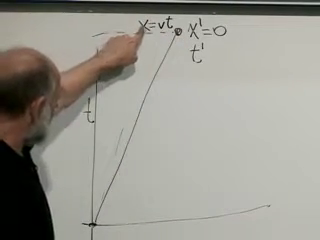
\includegraphics[width=0.72\textwidth]{lecture_04_figure_03.png}
\caption{L’origine mobile : $x=vt$, $x'=0$ et l’axe $t'$ sont trois descriptions d’une même ligne d’univers.}
\lectureframe{00:48:18}
\end{figure}

Appliquons l’intervalle invariant entre l’origine commune et un point ultérieur de cette ligne d’univers :
\begin{align}
t'^2-x'^2&=t^2-x^2,\\
t'^2&=t^2-v^2t^2,\\
t'&=t\sqrt{1-v^2}.
\label{eq:l4-time-dilation-natural}
\end{align}
En rétablissant $c$,
\begin{equation}
\Delta\tau=\Delta t\sqrt{1-\frac{v^2}{c^2}}
=\frac{\Delta t}{\gamma},
\qquad
\gamma=\frac{1}{\sqrt{1-v^2/c^2}}.
\label{eq:l4-time-dilation}
\end{equation}

\begin{figure}[H]
\centering
\includegraphics[width=0.73\textwidth]{lecture_04_figure_09.png}
\caption{Le résultat de dilatation du temps au tableau : l’horloge mobile accumule $t'=t\sqrt{1-v^2}$ dans les unités où $c=1$.}
\lectureframe{00:50:45}
\end{figure}

L’observateur immobile dit que l’horloge mobile retarde. Par réciprocité, l’observateur mobile doit dire la même chose des horloges immobiles. Il n’y a pas de contradiction, car les deux descriptions comparent des paires différentes d’événements éloignés.

En effet, une valeur constante de $t'$ dans l’équation~\eqref{eq:l4-lorentz-natural} vérifie
\begin{equation}
t-vx=\text{constant}.
\label{eq:l4-simultaneity}
\end{equation}
Les lignes de simultanéité de l’observateur mobile sont inclinées par rapport aux lignes horizontales $t=\text{constant}$. Chaque observateur considère comme simultanés des ensembles différents d’indications d’horloges éloignées. Dès lors que cette différence reste présente à l’esprit, le ralentissement réciproque des horloges est cohérent.

\begin{figure}[H]
\centering
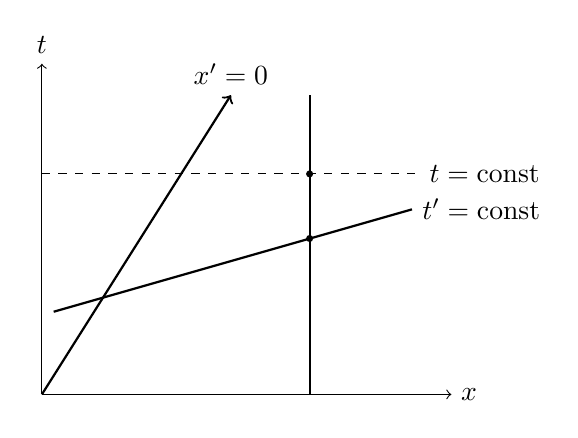
\begin{tikzpicture}[x=1cm,y=1cm]
\draw[->] (0,0) -- (0,4.2) node[above] {$t$};
\draw[->] (0,0) -- (5.2,0) node[right] {$x$};
\draw[thick,->] (0,0) -- (2.4,3.8) node[above] {$x'=0$};
\draw[dashed] (0,2.8) -- (4.8,2.8)
  node[right] {$t=\mathrm{const}$};
\draw[thick] (0.15,1.05) -- (4.7,2.35)
  node[right] {$t'=\mathrm{const}$};
\draw[thick] (3.4,0) -- (3.4,3.8);
\fill (3.4,2.8) circle (0.045);
\fill (3.4,1.98) circle (0.045);
\end{tikzpicture}
\caption{La dilatation réciproque du temps compare des indications d’horloges sur des tranches de simultanéité différentes.}
\end{figure}

\section{Les trajectoires des jumeaux}

Deux jumeaux partent du même événement. L’un reste en $x=0$. L’autre s’éloigne à la vitesse $v$, fait demi-tour et revient à la même vitesse. Lorsqu’ils se retrouvent, ils comparent tous les processus physiques pouvant servir d’horloge : montres, battements du cœur, métabolisme ou vieillissement lui-même.

Supposons que chaque moitié du voyage dure $T$ en temps coordonné dans le référentiel du jumeau resté chez lui. Son temps propre est
\begin{equation}
\tau_{\mathrm{home}}=2T.
\end{equation}
L’événement du demi-tour a pour coordonnées $(vT,T)$. La première étape du voyage contribue donc à
\begin{align}
\tau_{\mathrm{leg}}
&=\sqrt{T^2-v^2T^2}
=T\sqrt{1-v^2}.
\end{align}
L’étape du retour apporte la même durée, d’où
\begin{equation}
\tau_{\mathrm{travel}}=2T\sqrt{1-v^2}<2T.
\label{eq:l4-twin}
\end{equation}

\begin{figure}[H]
\centering
\includegraphics[width=0.73\textwidth]{lecture_04_figure_10.png}

\vspace{0.8em}

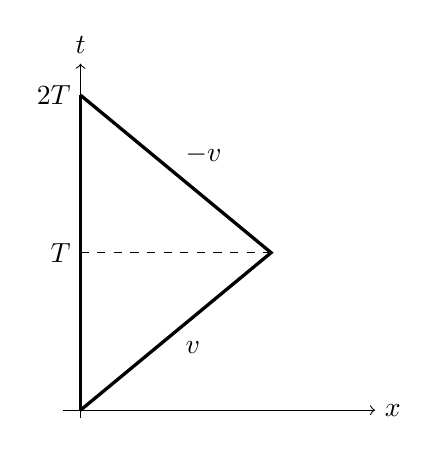
\begin{tikzpicture}[x=1.1cm,y=1cm]
\draw[->] (-0.2,0) -- (3.4,0) node[right] {$x$};
\draw[->] (0,-0.1) -- (0,4.4) node[above] {$t$};
\draw[very thick] (0,0) -- (0,4);
\draw[very thick] (0,0) -- (2.2,2) -- (0,4);
\draw[dashed] (0,2) -- (2.2,2);
\node[left] at (0,2) {$T$};
\node[left] at (0,4) {$2T$};
\node[below right] at (1.1,1.0) {$v$};
\node[above right] at (1.1,3.0) {$-v$};
\end{tikzpicture}\caption{La ligne d’univers du jumeau resté chez lui et les deux étapes du voyage. Leurs temps propres diffèrent parce que leurs trajectoires dans l’espace-temps sont différentes.}
\lectureframe{00:59:35}
\end{figure}

L’inégalité des âges n’a rien de contradictoire. La trajectoire du voyageur comporte un demi-tour et n’est pas liée à la ligne droite du jumeau resté chez lui par une unique symétrie de référentiel inertiel. En géométrie euclidienne ordinaire, un trajet rectiligne et un trajet brisé entre deux points ont également des longueurs différentes. La géométrie de Minkowski inverse la trajectoire dont l’intervalle est le plus grand, mais la comparaison reste géométrique.

\section{Accélération et horloge idéale}

\begin{classroomqa}\audiencequestion{Au moment du demi-tour, la situation physique est différente et le voyageur accélère. Cela invalide-t-il le calcul des horloges ?\lecturetimestamp{01:02:19}}\lecturerresponse{L’accélération est réelle et contribue à révéler l’asymétrie ; il ne faut pas chercher à l’écarter du raisonnement. Le coin pointu n’est qu’une représentation idéalisée et peut être arrondi en un demi-tour de durée finie. L’autre hypothèse physique est qu’une horloge suffisamment petite et bien conçue est insensible à une accélération modérée et continue de mesurer le temps propre. Une horloge grande ou fragile risque de se déformer ou de se briser, mais ce serait un défaut de son mécanisme, et non de l’intervalle d’espace-temps.}
\end{classroomqa}

Cette hypothèse de l’horloge idéale ne découle pas de la seule transformation de Lorentz. Elle est mise à l’épreuve par le comportement des mécanismes d’horlogerie réels. Un atome en constitue une bien meilleure approximation qu’une horloge large de plusieurs centaines de miles, car un mécanisme compact est plus difficile à déformer sous l’effet de l’accélération ou de la gravité. Invoquer la relativité générale ne résoudrait pas cette difficulté physique : il faudrait toujours savoir comment le mécanisme choisi réagit à son environnement.

\begin{classroomqa}\audiencequestion{Peut-on décomposer une trajectoire accélérée en courts intervalles sur lesquels l’analyse inertielle reste valable ?\lecturetimestamp{01:09:08}}\lecturerresponse{Oui. Découpons la courbe en segments courts, presque rectilignes, calculons le temps propre sur chaque segment, puis additionnons les résultats. C’est l’analogue dans l’espace-temps du calcul de la longueur d’une courbe ordinaire à partir d’une multitude de petits segments de droite. À la limite continue,
\[
\tau=\int \sqrt{1-\frac{v(t)^2}{c^2}}\,dt,
\]
pour un mouvement dans un espace-temps plat décrit dans un système de coordonnées inertiel.}
\end{classroomqa}

\section{Ce que voient les jumeaux}

On peut rendre opérationnelles les indications finales des horloges en envoyant des impulsions lumineuses. Marquons des intervalles de temps propre d’une seconde sur les deux lignes d’univers et faisons émettre une impulsion par chaque jumeau à chaque marque. Pendant l’étape de l’aller, les impulsions reçues de l’autre jumeau sont de plus en plus espacées. Au retour, elles arrivent de plus en plus rapprochées. C’est l’effet Doppler relativiste représenté directement sur le diagramme d’espace-temps.

\begin{figure}[H]
\centering
\includegraphics[width=0.73\textwidth]{lecture_04_figure_11.png}
\caption{Signaux lumineux échangés entre la ligne d’univers du jumeau resté chez lui et celle du voyageur. Les arrivées espacées pendant l’aller puis rapprochées pendant le retour rendent compte de toutes les impulsions émises.}
\lectureframe{01:12:55}
\end{figure}

Aucune partie de l’histoire ne disparaît. Chaque observateur finit par recevoir toutes les impulsions émises par l’autre, mais leur fréquence de réception dépend du mouvement relatif. Les effets de décalage vers le rouge à l’aller et vers le bleu au retour n’ont pas la même durée pour les deux trajectoires ; le décompte de toutes les impulsions reçues concorde donc avec la comparaison des temps propres.

\begin{classroomqa}\audiencequestion{Si le voyageur de retour reçoit une lumière décalée vers le bleu, pourrait-il recueillir plus d’énergie que la source n’en a émise ?\lecturetimestamp{01:13:50}}\lecturerresponse{Pour répondre, il faut avoir développé la définition relativiste de l’énergie et sa dépendance au référentiel. La question est légitime, mais les coordonnées et le décompte des impulsions ne suffisent pas à établir le bilan énergétique, surtout pour un observateur accéléré. Il vaut donc mieux différer la réponse que la deviner.}
\end{classroomqa}

\section{Une direction spatiale fermée}

\begin{classroomqa}\audiencequestion{Supposons qu’une direction spatiale soit compacte. Un jumeau pourrait-il s’y déplacer uniformément, revenir à son point de départ et éviter toute accélération ? Qu’est-ce qui distinguerait alors les jumeaux ?\lecturetimestamp{01:15:14}}\lecturerresponse{Il faut concevoir l’espace intrinsèquement comme un cylindre, et non comme une feuille courbée dans un espace plus vaste ; il n’y a pas nécessairement d’accélération radiale. L’observateur qui revient rencontre néanmoins le fait global que les mêmes lieux se répètent. Cela indique une asymétrie, mais une réponse complète exige un traitement rigoureux de la relativité restreinte avec l’identification spatiale. Nous laissons ici la question ouverte au lieu d’improviser une réponse.}
\end{classroomqa}

\begin{figure}[H]
\centering
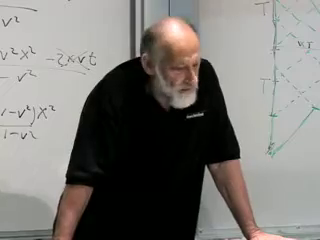
\includegraphics[width=0.72\textwidth]{lecture_04_figure_04.png}

\vspace{0.8em}

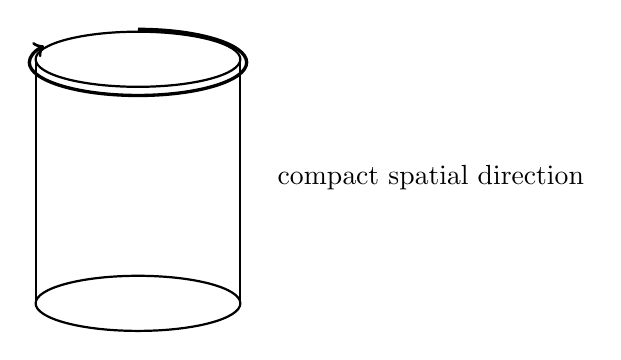
\begin{tikzpicture}[x=1cm,y=1cm]
\draw[thick] (0,0) ellipse (1.3 and 0.35);
\draw[thick] (-1.3,0) -- (-1.3,-3.1);
\draw[thick] (1.3,0) -- (1.3,-3.1);
\draw[thick] (0,-3.1) ellipse (1.3 and 0.35);
\draw[->,very thick] (0.0,0.38) arc (90:-210:1.38 and 0.42);
\node[right] at (1.65,-1.5) {compact spatial direction};
\end{tikzpicture}\caption{La question de l’espace compact telle qu’elle est dessinée au tableau, avec un cylindre intrinsèque net. Elle porte sur une identification globale, et non sur un mouvement autour d’un cylindre plongé dans une dimension radiale supplémentaire.}
\lectureframe{01:17:56}
\end{figure}

\section{La longueur se mesure sur une tranche de simultanéité}

Pour un problème de relativité restreinte, commençons par dessiner le diagramme d’espace-temps. Prenons une règle d’un mètre au repos dans le référentiel non primé, dont les extrémités se trouvent en $x=0$ et $x=1$. Au fil du temps, les deux extrémités décrivent des lignes d’univers verticales. La règle balaie un ruban dans l’espace-temps.

L’observateur mobile doit mesurer les deux extrémités à une même valeur du temps mobile $t'$. D’après l’équation~\eqref{eq:l4-simultaneity}, la tranche qui passe par l’origine et vérifie $t'=0$ satisfait
\begin{equation}
t=vx
\end{equation}
dans les unités où $c=1$. Elle coupe la ligne d’univers de l’extrémité droite $x=1$ en $t=v$.

\begin{figure}[H]
\centering
\includegraphics[width=0.73\textwidth]{lecture_04_figure_12.png}

\vspace{0.8em}

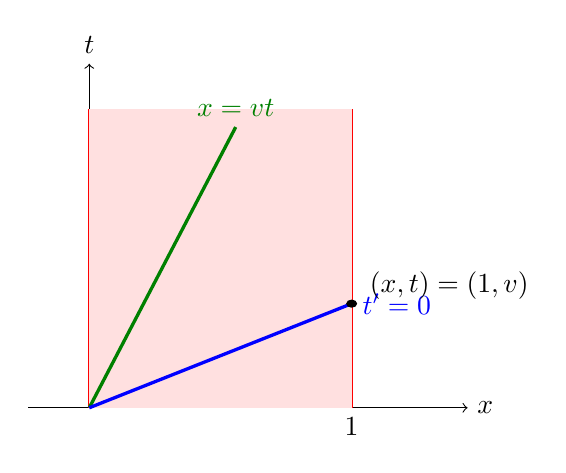
\begin{tikzpicture}[x=1.55cm,y=1.15cm]
\draw[->] (-0.5,0) -- (3.1,0) node[right] {$x$};
\draw[->] (0,0) -- (0,3.8) node[above] {$t$};
\draw[very thick,red] (0,0) -- (0,3.3);
\draw[very thick,red] (2.15,0) -- (2.15,3.3);
\fill[red!12] (0,0) rectangle (2.15,3.3);
\draw[very thick,green!50!black] (0,0) -- (1.2,3.1)
  node[above] {$x=vt$};
\draw[very thick,blue] (0,0) -- (2.15,1.15)
  node[right] {$t'=0$};
\fill (2.15,1.15) circle (0.045);
\node[right] at (2.22,1.35) {$(x,t)=(1,v)$};
\node[below] at (2.15,0) {$1$};
\end{tikzpicture}\caption{Une règle au repos balaie un ruban dans l’espace-temps. Pour l’observateur mobile, la longueur est la distance entre ses extrémités sur une tranche $t'=\mathrm{const}$.}
\lectureframe{01:24:20}
\end{figure}

La séparation choisie entre les extrémités est de genre espace ; utilisons donc la forme spatiale positive de l’invariant :
\begin{equation}
x'^2-t'^2=x^2-t^2.
\end{equation}
À l’extrémité choisie, $t'=0$, $x=1$ et $t=v$. On a donc
\begin{align}
x'^2&=1-v^2,\\
x'&=\sqrt{1-v^2}.
\end{align}
Ainsi, une longueur au repos $L$ est mesurée dans le référentiel mobile comme
\begin{equation}
L'=L\sqrt{1-v^2/c^2}=\frac{L}{\gamma}.
\label{eq:l4-length-contraction}
\end{equation}

\begin{figure}[H]
\centering
\includegraphics[width=0.76\textwidth]{lecture_04_figure_13.png}
\caption{La construction complète de la contraction des longueurs et le résultat au tableau $x'=\sqrt{1-v^2}$ pour une longueur au repos unitaire.}
\lectureframe{01:28:10}
\end{figure}

La réciproque est également vraie : l’observateur sur le quai attribue une longueur plus courte à la règle longitudinale d’un mètre du train. Une fois encore, les deux observateurs choisissent des événements simultanés différents aux extrémités, si bien que cette réciprocité n’est pas contradictoire.

\section{Questions de fin de cours}

\begin{classroomqa}
\audiencequestion{À part la lumière, quelque chose se propage-t-il à la vitesse de la lumière ? Qu’en est-il en particulier de la gravité ?\lecturetimestamp{01:29:29}}
\lecturerresponse{La relativité générale prédit que les ondes gravitationnelles se propagent à $c$. À l’époque de ce cours, les indices étaient indirects et provenaient de systèmes tels que les pulsars binaires ; les ondes gravitationnelles n’avaient pas encore été détectées directement.\editorialnote{La situation expérimentale a changé après ce cours de 2006. LIGO a détecté directement GW150914 en 2015, et l’observation conjointe de GW170817 et de son homologue électromagnétique en 2017 a montré que les vitesses de propagation de la gravité et de la lumière concordent à quelques parties près sur $10^{15}$. Voir \url{https://ligo.org/detections/gw150914/} et
\url{https://doi.org/10.1103/PhysRevLett.119.251302}.}}
\end{classroomqa}

\begin{classroomqa}\audiencequestion{Un astronaute peut-il parcourir une distance de plusieurs années-lumière en un temps propre inférieur à cette distance exprimée en années-lumière ? Cela signifierait-il qu’il se déplace plus vite que la lumière ?\lecturetimestamp{01:30:38}}\lecturerresponse{Le temps propre de l’astronaute est $\sqrt{\Delta t^2-\Delta x^2}$, une durée inférieure au temps coordonné $\Delta t$. Dans le référentiel inertiel de l’astronaute, la distance entre les étoiles est contractée par Lorentz. Les étoiles se déplacent à la vitesse $-v$, et non plus vite que la lumière ; la distance à parcourir est simplement plus courte après contraction.}
\end{classroomqa}

Si l’astronaute part du repos et accélère, la description change au fil d’une succession de référentiels inertiels instantanés. La distance attribuée aux étoiles peut varier pendant cette transition. On ne peut pas appliquer une unique transformation de Lorentz à toute l’histoire accélérée, mais le temps propre total s’obtient toujours en additionnant les contributions le long de la ligne d’univers. Il en va de même pour un jumeau réaliste qui démarre, fait demi-tour et décélère, au lieu de naître à la vitesse de croisière.

\begin{classroomqa}\audiencequestion{Ces paradoxes viennent-ils du fait que le temps est traité comme une notion particulière ? Faut-il parler d’une quatrième dimension ?\lecturetimestamp{01:36:43}}\lecturerresponse{Il n’est pas nécessaire de commencer par affirmer que le temps est une quatrième dimension. La transformation de Lorentz impose à elle seule le mélange de l’espace et du temps, tandis que l’intervalle $t^2-x^2-y^2-z^2$ les traite comme des composantes d’une même géométrie, avec un signe différent pour le temps et pour l’espace. À faible vitesse, le mélange devient négligeable et l’intuition newtonienne familière reprend ses droits. Aux vitesses relativistes, en revanche, on ne peut pas considérer l’espace et le temps comme fondamentalement découplés.}
\end{classroomqa}

La dilatation du temps, la contraction des longueurs, la comparaison des jumeaux et la réduction du temps de voyage ne sont donc pas des astuces distinctes. Elles découlent toutes de trois habitudes : repérer les événements comparés, représenter leur géométrie dans l’espace-temps et utiliser l’intervalle invariant.